% last updated to inet commit 'e10ce09097652b72f41fcbde5dc81a2cc2537d32'

\chapter{Node Mobility}
\label{cha:mobility}


\section{Overview}

In order to accurately evaluate a protocol for an ad-hoc network,
it is important to use a realistic model for the motion of mobile
hosts. Signal strengths, radio interference and channel occupancy
depends on the distances between nodes. The choice of the mobility
model can significantly influence the results of a simulation
(e.g. data packet delivery ratio, end-to-end delay, average hop count)
as shown in \cite{Camp02asurvey}.

There are two methods for incorporating mobility into simulations:
using traces and synthetic models. Traces contains recorded motion
of the mobile hosts, as observed in real life system. Synthetic models
use mathematical models for describing the behaviour of the mobile hosts.

There are mobility models that represent mobile nodes whose movements
are independent of each other (entity models) and mobility models
that represent mobile nodes whose movements are dependent on each other
(group models). Some of the most frequently used entity models are the
Random Walk Mobility Model, Random Waypoint Mobility Model, Random
Direction Mobility Model, Gauss-Markov Mobility Model, City Section
Mobility Model. The group models include the Column Mobility Model,
Nomadic Community Mobility Model, Pursue Mobility Model,
Reference Point Group Mobility Model.

The INET framework has components for the following trace files:

\begin{itemize}
\item \tbf{Bonn Motion} native file format of the
    \href{http://net.cs.uni-bonn.de/wg/cs/applications/bonnmotion/}{BonnMotion}
    scenario generation tool.
\item \tbf{Ns2} trace file generated by the CMU's scenario generator that used in Ns2.
\item \tbf{ANSim} XML trace file of the ANSim (Ad-Hoc Network Simulation) tool.
\end{itemize}

It is easy to integrate new entity mobility models into the INET framework,
but group mobility is not supported yet. Therefore all the models
shipped with INET are implementations of entitiy models:

\begin{itemize}
\item \tbf{Deterministic Motions} for fixed position nodes and nodes
      moving on a linear, circular, rectangular paths.
\item \tbf{Random Waypoint} model includes pause times between changes
      in destination and speed.
\item \tbf{Gauss-Markov} model uses one tuning parameter to vary the degree
      of randomness in mobility pattern.
\item \tbf{Mass Mobility} models a mass point with inertia and momentum.
\item \tbf{Chiang Mobility} uses a probabilistic transition matrix to change
      the state of motion of the node.
\end{itemize}

\section{Mobility in INET}

In INET mobile nodes have to contain a module implementing the
\nedtype{IMobility} marker interface. This module stores the current
coordinates of the node and is responsible for updating the position
periodically and emitting the \ttt{mobilityStateChanged} signal
when the position changed.

The p[0] and p[1] fields of the display string of the node is
also updated, so if the simulation run is animated, the node is
actually moving on the screen. The current position of the node
can be obtained from the display string.

The radio simulations has a \nedtype{ChannelControl} module that takes case of
establishing communication channels between nodes that are within
communication distance and tearing down the connections when they
move out of range. The \nedtype{ChannelControl} module uses to
\ttt{mobilityStateChanged} signal to determine when the connection
status needs to be updated.

There are two possibilities to implement a new mobility model. The simpler but
limited one is to use \nedtype{TurtleMobility} as the mobility component and to
write a script similar to the turtle graphics of LOGO. The second is to
implement a simple module in C++. In this case the C++ class of the mobility
module should be derived from \cppclass{IMobility} and its NED type should
implement the \nedtype{IMobility} interface.

%\begin{figure}
%\begin{center}
%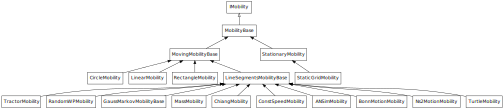
\includegraphics{figures/mobility_classes}
%\end{center}
%\end{figure}

% FIXME The Z coordinate is often initialized randomly.
%       It would be better (backward compatibility)
%       to initialize them to 0. (contsraintAreaDepth=0 not handled everywhere)

\subsection{MobilityBase class}

The abstract \cppclass{MobilityBase} class is the base of the mobility
modules defined in the INET framework. This class allows to define
a cubic volume that the node can not leave. The volume is configured
by setting the \fpar{constraintAreaX}, \fpar{constraintAreaY},
\fpar{constraintAreaZ},
\fpar{constraintAreaWidth}, \fpar{constraintAreaHeight} and
\fpar{constraintAreaDepth} parameters.

When the module is initialized it sets the initial position of the node
by calling the \ffunc{initializePosition()} method.
The default implementation of this method sets the position from the
display string if the \fpar{initFromDisplayString} parameter is true.
Otherwise the position can be given as the \fpar{initialX},
\fpar{initialY} and \fpar{initialZ} parameters.
If neither of these parameters are given,
a random initial position is choosen within the contraint area.

The module is responsible for periodically updating the position.
For this purpose it should send timer messages to itself. These messages
are processed in the \ffunc{handleSelfMessage} method. In derived
classes, \ffunc{handleSelfMessage} should compute the new position
and update the display string and publish the new position by calling
the \ffunc{positionUpdated} method.

When the node reaches the boundary of the constraint area, the mobility
component has to prevent the node to exit. It can call the
\ffunc{handleIfOutside} method, that offers the following policies:

\begin{itemize}
  \item reflect of the wall
  \item reappear at the opposite edge (torus area)
  \item placed at a randomly chosen position of the area
  \item stop the simulation with an error
\end{itemize}

\subsection{MovingMobilityBase}

The abstract \cppclass{MovingMobilityBase} class can be used to model
mobilities when the node moves on a continous trajectory and
updates its position periodically. Subclasses only need to implement
the \ffunc{move} method that is responsible to update the current
position and speed of the node.

The abstract \ffunc{move} method is called autmotically in every
\fpar{updateInterval} steps. The method is also called when a client
requested the current position or speed or when the \ffunc{move} method
requested an update at a future moment by setting the \fvar{nextChange}
field. This can be used when the state of the motion changes at a
specific time that is not a multiple of \fpar{updateInterval}.
The method can set the \fpar{stationary} field to \ttt{true} to
indicate that the node reached its final position and no more position
update is needed.

% TODO draw a plot of t-position function marking the points when
%      move() is called, stationary set to true, etc.

\subsection{LineSegmentsMobilityBase}

The path of a mobile node often consist of linear movements of constant
speed. The node moves with some speed for some time, then with another
speed for another duration and so on. If a mobility model fits this
description, it might be suitable to derive the implementing C++ class
from \cppclass{LineSegmentsMobilityBase}.

The module first choose a target position and a target time by calling
the \ffunc{setTargetPosition} method. If the target position differs
from the current position, it starts to move toward the target and
updates the position in the configured \fpar{updateInterval} intervals.
When the target position reached, it chooses a new target.

% TODO draw a plot like above, but containing linear segments, mark
%      the points when setTargetPosition called.

% FIXME LineSegmentsMobilityBase should not schedule the self message at updateInterval
%       when lastPosition==targetPosition (the node is waiting at the current position,
%       e.g. every second step in RandomWPMobility)
% TODO Consider an updateInterval computed from an updateDistance and speed, because position change
%      may be irrevelant during a preconfigured updateInterval.

\section{Implemented models}

\subsection{Deterministic movements}

\begin{description}

\item[StationaryMobility] This mobility module does nothing;
it can be used for stationary nodes.

\item[StaticGridMobility] Places all nodes in a rectangular grid.

% TODO it always creates an N x N grid, generalize

\item[LinearMobility] This is a linear mobility model with speed,
angle and acceleration parameters. Angle only changes when the mobile
node hits a wall: then it reflects off the wall at the same angle.

z coordinate is constant
movement is always parallel with X-Y plane

% TODO interpret 'angle' as asimuth and introduce inclination angle (default is 0)
%      to describe movement along arbitrary line segment
% FIXME why different speed and lastSpeed

\item[CircleMobility] Moves the node around a circle parallel to the X-Y plane
with constant speed.
The node bounces from the bounds of the constraint area.
The circle is given by the \fpar{cx}, \fpar{cy} and \fpar{r} parameters,
The initial position determined by the \fpar{startAngle} parameter.
The position of the node is refreshed in \fpar{updateInterval} steps.

\item[RectangleMobility] Moves the node around the constraint area.
configuration: speed, startPos, updateInterval
% should be derived from LineSegmentsMobilityBase?

\item[TractorMobility] Moves a tractor through a field with a certain
amount of rows. The following figure illustrates the movement of the
tractor when the \fpar{rowCount} parameter is 2. The trajectory follows
the segments in $1,2,3,4,5,6,7,8,1,2,3\ldots$ order. The area is configured
by the \fpar{x1}, \fpar{y1}, \fpar{x2}, \fpar{y2} parameters.

% TODO use constraint area instead of new x1,y1,x2,y2 parameters as in RectangleMobility

\begin{center}
\setlength{\unitlength}{0.5mm}
\begin{picture}(80,80)
\put(40,72){$1$} \put(10,70){\vector(1,0){30}} \put(10,70){\line(1,0){60}}
\put(72,55){$2$} \put(70,70){\vector(0,-1){15}} \put(70,70){\line(0,-1){30}}
\put(40,42){$3$} \put(70,40){\vector(-1,0){30}} \put(70,40){\line(-1,0){60}}
\put(5,25){$4$} \put(10,40){\vector(0,-1){15}} \put(10,40){\line(0,-1){30}}
\put(40,12){$5$} \put(10,10){\vector(1,0){30}} \put(10,10){\line(1,0){60}}
\put(72,25){$6$} \put(70,10){\vector(0,1){15}} \put(70,10){\line(0,1){30}}
\put(40, 33){$7$}
\put(5,55){$8$} \put(10,40){\vector(0,1){15}} \put(10,40){\line(0,1){30}}
\put(0,72){$(x_1,y_1)$} \put(65,2){$(x_2,y_2)$}
\end{picture}
\end{center}

\end{description}

\subsection{Random movements}

\begin{description}

\item[RandomWPMobility]

In the Random Waypoint mobility model the nodes move in line segments. For each
line segment, a random destination position (distributed uniformly over the
playground) and a random speed is chosen. You can define a speed as a variate
from which a new value will be drawn for each line segment; it is customary to
specify it as \ttt{uniform(minSpeed, maxSpeed)}. When the node reaches the
target position, it waits for the time \fpar{waitTime} which can also be defined as a
variate. After this time the the algorithm calculates a new random position, etc.

\item[GaussMarkovMobility] The Gauss-Markov model contains a tuning
parameter, that control the randomness in the movement of the node.
Let the magnitude and direction of speed of the node at the $n$th time step be
$s_n$ and $d_n$. The next speed and direction is computed as

$$ s_{n+1} = \alpha s_n + (1 - \alpha) \bar{s} +
             \sqrt{(1-\alpha^2)} s_{x_n} $$

$$ d_{n+1} = \alpha s_n + (1 - \alpha) \bar{d} +
             \sqrt{(1-\alpha^2)} d_{x_n} $$

where $\bar{s}$ and $\bar{d}$ are constants representing the mean value
of speed and direction as $n \to \infty$; and $s_{x_n}$ and $d_{x_n}$
are random variables with Gaussian distribution.

Totally random walk (Brownian motion) is obtained by setting $\alpha=0$,
while $\alpha=1$ results a linear motion.

To ensure that the node does not remain at the boundary of the constraint
area for a long time, the mean value of the direction ($\bar{d}$) modified
as the node enters the margin area. For example at the right edge of the
area it is set to 180 degrees, so the new direction is away from the edge.

% FIXME the GaussMarkovMobility module has only one variance parameter.
%       it should have separate speed and direction parameters

\item[MassMobility]

This is a random mobility model for a mobile host with
a mass. It is the one used in \cite{Perkins99optimizedsmooth}.

\begin{quote}
"An MH moves within the room according to the following pattern. It moves
along a straight line for a certain period of time before it makes a turn.
This moving period is a random number, normally distributed with average of
5 seconds and standard deviation of 0.1 second. When it makes a turn, the
new direction (angle) in which it will move is a normally distributed
random number with average equal to the previous direction and standard
deviation of 30 degrees. Its speed is also a normally distributed random
number, with a controlled average, ranging from 0.1 to 0.45 (unit/sec), and
standard deviation of 0.01 (unit/sec). A new such random number is picked
as its speed when it makes a turn. This pattern of mobility is intended to
model node movement during which the nodes have momentum, and thus do not
start, stop, or turn abruptly. When it hits a wall, it reflects off the
wall at the same angle; in our simulated world, there is little other
choice."
\end{quote}

This implementation can be parameterized a bit more, via the
\fpar{changeInterval}, \fpar{changeAngleBy} and \fpar{changeSpeedBy} parameters.
The parameters described above correspond to the following settings:

\begin{inifile}
changeInterval = normal(5, 0.1)
changeAngleBy = normal(0, 30)
speed = normal(avgSpeed, 0.01)
\end{inifile}

\item[ChiangMobility] Chiang's random walk movement model
(\cite{Chiang98wirelessnetwork}).

In this model, the state of the mobile node in each direction (x and y) can be:

\begin{itemize}
  \item 0: the node stays in its current position
  \item 1: the node moves forward
  \item 2: the node moves backward
\end{itemize}

The $(i,j)$ element of the state transition matrix determines the
probability that the state changes from $i$ to $j$:

$$ \left(
\begin{array}{ccc}
  0 & 0.5 & 0.5 \\
  0.3 & 0.7 & 0 \\
  0.3 & 0 & 0.7
\end{array}
\right) $$

The \nedtype{ChiangMobility} module supports the following parameters:
\begin{itemize}
  \item \fpar{updateInterval} position update interval
  \item \fpar{stateTransitionInterval} state update interval
  \item \fpar{speed}: the speed of the node
\end{itemize}


% FIXME last line of setTargetPosition() contains a sign error, should be
%              targetPosition = lastPosition + lastSpeed * stateTransitionUpdateInterval;
% FIXME when reflecting at the boundary, state variables should be reflected too

\item[ConstSpeedMobility]

\nedtype{ConstSpeedMobility} does not use one of the standard mobility
approaches. The user can define a velocity for each Host and an update interval. If
the velocity is greater than zero (i.e. the Host is not stationary) the
\nedtype{ConstSpeedMobility} module calculates a random target position for the
Host. Depending to the update interval and the velocity it calculates the number of
steps to reach the destination and the step-size. Every update interval
\nedtype{ConstSpeedMobility} calculates the new position on its way to the
target position and updates the display. Once the target position is reached
\nedtype{ConstSpeedMobility} calculates a new target position.

This component has been taken over from Mobility Framework 1.0a5.

% FIXME this is a special case of RandomWPMobility, remove

\end{description}

\subsection{Replaying trace files}

\begin{description}

\item[BonnMotionMobility] Uses the native file format of
\href{http://www.cs.uni-bonn.de/IV/BonnMotion/}{BonnMotion}.

The file is a plain text file, where every line describes the motion
of one host. A line consists of one or more (t, x, y) triplets of real
numbers, like:

\begin{verbatim}
t1 x1 y1 t2 x2 y2 t3 x3 y3 t4 x4 y4 ...
\end{verbatim}

The meaning is that the given node gets to $(xk,yk)$ at $tk$. There's no
separate notation for wait, so x and y coordinates will be repeated there.

\item[Ns2Mobility] Nodes are moving according to the trace files used
in NS2.
The trace file has this format:

\begin{verbatim}
# '#' starts a comment, ends at the end of line
$node_(<id>) set X_ <x> # sets x coordinate of the node identified by <id>
$node_(<id>) set Y_ <y> # sets y coordinate of the node identified by <id>
$node_(<id>) set Z_ <z> # sets z coordinate (ignored)
$ns at $time "$node_(<id>) setdest <x> <y> <speed>" # at $time start moving
towards <x>,<y> with <speed>
\end{verbatim}

The \nedtype{Ns2MotionMobility} module has the following parameters:

\begin{itemize}
  \item \fpar{traceFile} the Ns2 trace file
  \item \fpar{nodeId} node identifier in the trace file; -1 gets substituted by
  parent module's index
  \item \fpar{scrollX},\fpar{scrollY} user specified translation of the
  coordinates
\end{itemize}

% TODO cleaning the code (e.g. duplicated bounds check in setTargetPosition())
% TODO implement cached file access as in BonnMotionMobility

\item[ANSimMobility] reads trace files of the \href{http://www.ansim.info}{ANSim} Tool.

The nodes are moving along linear segments described by an XML trace file
conforming to this DTD:

\begin{verbatim}
<!ELEMENT mobility (position_change*)>
<!ELEMENT position_change (node_id, start_time, end_time, destination)>
<!ELEMENT node_id (#PCDATA)>
<!ELEMENT start_time (#PCDATA)>
<!ELEMENT end_time (#PCDATA)>
<!ELEMENT destination (xpos, ypos)>
<!ELEMENT xpos (#PCDATA)>
<!ELEMENT ypos (#PCDATA)>
\end{verbatim}

Parameters of the module:

\begin{itemize}
  \item \fpar{ansimTrace} the trace file
  \item \fpar{nodeId} the \verb!node_id! of this node, -1 gets substituted to
  parent module's index
\end{itemize}

\begin{note}
The \nedtype{ANSimMobility} module process only the \ttt{position\_{}change}
elements and it ignores the \ttt{start\_{}time} attribute. It starts the move
on the next segment immediately.
\end{note}


\end{description}




\section{Mobility scripts}

The \nedtype{TurtleMobility} module can be parametrized by a script file
containing LOGO-style movement commands in XML format.

The module has these parameters:

\begin{itemize}
\item \ttt{updateInterval} time interval to update the hosts position
\item \ttt{constraintAreaX}, \ttt{constraintAreaY}, \ttt{constraintAreaWidth},
      \ttt{constraintAreaHeight}: constraint area that the node can not leave
\item \ttt{turtleScript} XML file describing the movements
\end{itemize}

The content of the XML file should conform to the following DTD (can be
found as \ffilename{TurtleMobility.dtd} in the source tree):

\begin{verbatim}
<!ELEMENT movements (movement)*>

<!ELEMENT movement (repeat|set|forward|turn|wait|moveto|moveby)*>
<!ATTLIST movement id NMTOKEN #IMPLIED>

<!ELEMENT repeat (repeat|set|forward|turn|wait|moveto|moveby)*>
<!ATTLIST repeat n CDATA #IMPLIED>

<!ELEMENT set EMPTY>
<!ATTLIST set x     CDATA #IMPLIED
              y     CDATA #IMPLIED
              speed CDATA #IMPLIED
              angle CDATA #IMPLIED
              borderPolicy (reflect|wrap|placerandomly|error) #IMPLIED>

<!ELEMENT forward EMPTY>
<!ATTLIST forward d CDATA #IMPLIED
                  t CDATA #IMPLIED>

<!ELEMENT turn EMPTY>
<!ATTLIST turn angle CDATA #REQUIRED>

<!ELEMENT wait EMPTY>
<!ATTLIST wait t CDATA #REQUIRED>

<!ELEMENT moveto EMPTY>
<!ATTLIST moveto x CDATA #IMPLIED
                 y CDATA #IMPLIED
                 t CDATA #IMPLIED>

<!ELEMENT moveby EMPTY>
<!ATTLIST moveby x CDATA #IMPLIED
                 y CDATA #IMPLIED
                 t CDATA #IMPLIED>
\end{verbatim}

The file contains \ttt{movement} elements, each describing a trajectory.
The \ttt{id} attribute of the \ttt{movement} element can be used to
refer the movement from the ini file using the syntax:

\begin{inifile}
**.mobility.turtleScript = xmldoc("turtle.xml", "movements//movement[@id='1']")
\end{inifile}

The motion of the node is composed of uniform linear segments.
The state of motion is described by the following variables:
\begin{itemize}
\item \ttt{position}: $(x,y)$ coordinate of the current location of the node
\item \ttt{speed}, \ttt{angle}: magnitude and direction of the node's velocity
\item \ttt{targetPos}: target position of the current line segment. If given
                       the \ttt{speed} and \ttt{angle} is not used
\item \ttt{targetTime} the end time of the current linear motion
\item \ttt{borderPolicy}: one of
    \begin{itemize}
      \item \ttt{reflect} the node reflects at the boundary,
      \item \ttt{wrap} the node appears at the other side of the area,
      \item \ttt{placerandomly} the node placed at a random position of the area,
      \item \ttt{error} signals an error when the node reaches the boundary
    \end{itemize}
\end{itemize}

The \ttt{movement} elements may contain the the following commands:

\begin{itemize}
\item \ttt{repeat(n)} repeats its content n times, or indefinetly if the n attribute
              is omitted.
\item \ttt{set(x,y,speed,angle,borderPolicy)} modifies the state of the node.
\item \ttt{forward(d,t)} moves the node for $t$ time or to the $d$ distance
with the current speed. If both $d$ and $t$ is given, then the current
speed is ignored.
\item \ttt{turn(angle)} increase the angle of the node by $angle$ degrees.
\item \ttt{moveto(x,y,t)} moves to point $(x,y)$ in the given time. If
$t$ is not specified, it is computed from the current speed.
\item \ttt{moveby(x,y,t)} moves by offset $(x,y)$ in the given time. If
$t$ is not specified, it is computed from the current speed.
\item \ttt{wait(t)} waits for the specified amount of time.
\end{itemize}

Attribute values must be given without physical units, distances are assumed
to be given as meters, time intervals in seconds and speeds in meter per seconds.
Attibutes can contain expressions that are evaluated each time the
command is executed. The limits of the constraint area can be
referenced as \verb!$MINX!, \verb!$MAXX!, \verb!$MINY!, and \verb!$MAXY!.
Random number distibutions generate a new random number when evaluated,
so the script can describe random as well as deterministic scenarios.

To illustrate the usage of the module, we show how some mobility
models can be implemented as scripts:

\begin{itemize}
\item RectangleMobility:

\begin{verbatim}
    <movement>
        <set x="$MINX" y="$MINY" angle="0" speed="10"/>
        <repeat>
            <repeat n="2">
                <forward d="$MAXX-$MINX"/>
                <turn angle="90"/>
                <forward d="$MAXY-$MINY"/>
                <turn angle="90"/>
            </repeat>
        </repeat>
    </movement>
\end{verbatim}

\item Random Waypoint:

\begin{verbatim}
    <movement>
        <repeat>
            <set speed="uniform(20,60)"/>
            <moveto x="uniform($MINX,$MAXX)" y="uniform($MINY,$MAXY)"/>
            <wait t="uniform(5,10)">
        </repeat>
    </movement>
\end{verbatim}

\item MassMobility:

\begin{verbatim}
    <movement>
        <repeat>
            <set speed="uniform(10,20)"/>
            <turn angle="uniform(-30,30)"/>
            <forward t="uniform(0.1,1)"/>
        </repeat>
    </movement>
\end{verbatim}

\end{itemize}


%%% Local Variables:
%%% mode: latex
%%% TeX-master: "usman"
%%% End:


